% Sinh bởi report_figures/ve_hinh.py; hình vẽ ở kích thước in, chèn không co giãn.
% Đối chiếu với mã ai-service ngày 22/10/2026.

\begin{figure}[htbp]
  \centering
  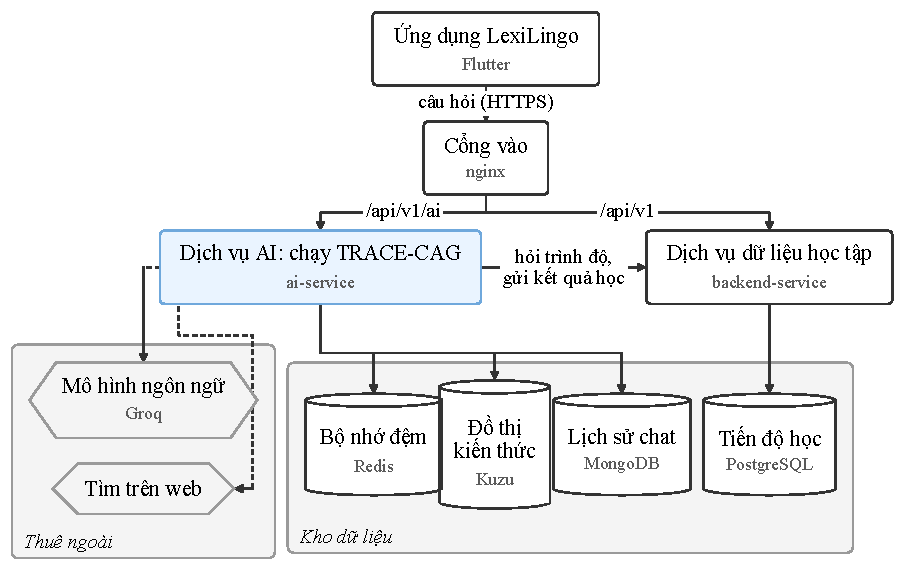
\includegraphics{figures/tracecag/h01_kien_truc.pdf}
  \caption{TRACE-CAG nằm trong dịch vụ AI; dữ liệu học tập do backend-service giữ. Nét đứt là dịch vụ thuê ngoài.}
  \label{fig:tc-kientruc}
\end{figure}

\begin{figure}[htbp]
  \centering
  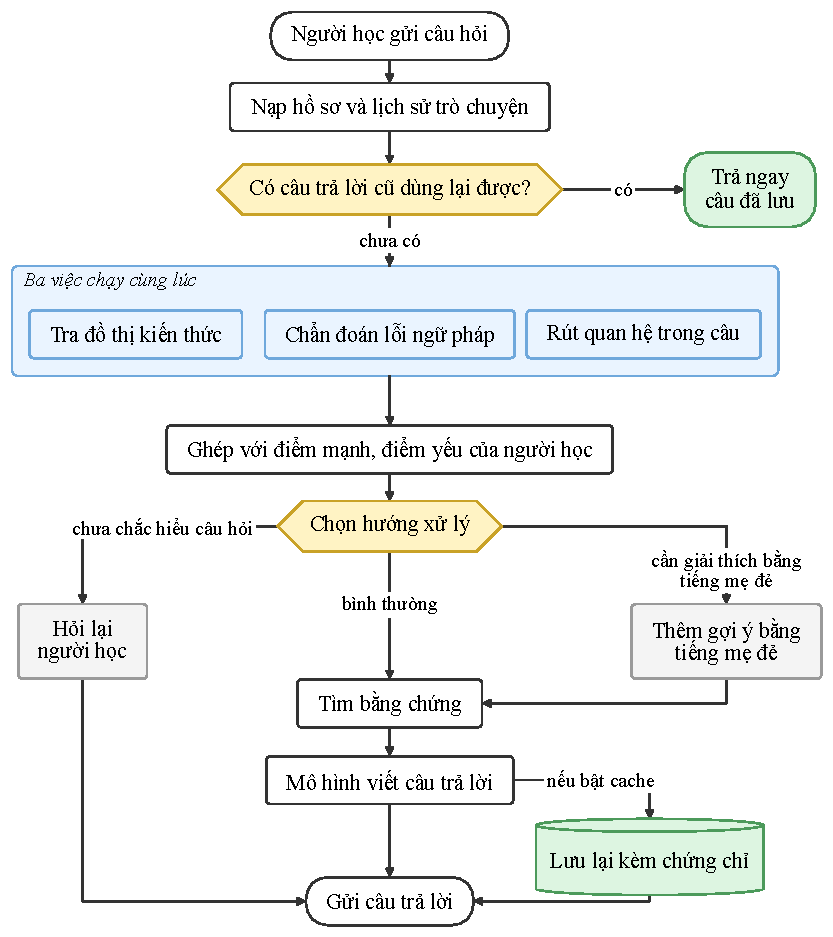
\includegraphics{figures/tracecag/h02_langgraph.pdf}
  \caption{Một câu hỏi đi qua TRACE-CAG: dùng lại câu cũ nếu được, nếu không thì phân tích, tìm bằng chứng, viết và lưu câu trả lời.}
  \label{fig:tc-langgraph}
\end{figure}

\begin{figure}[htbp]
  \centering
  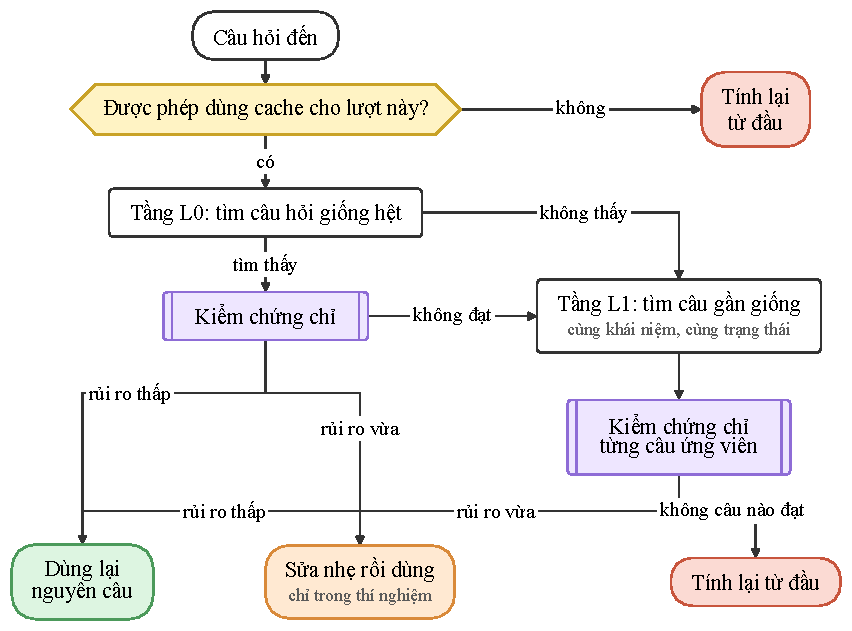
\includegraphics{figures/tracecag/h03_cong_cache.pdf}
  \caption{Cổng cache tìm câu cũ ở tầng L0 (giống hệt) rồi L1 (gần giống); câu nào tìm được cũng phải qua kiểm chứng chỉ. Sửa nhẹ (PATCH) chỉ xảy ra trong thí nghiệm.}
  \label{fig:tc-congcache}
\end{figure}

\begin{figure}[htbp]
  \centering
  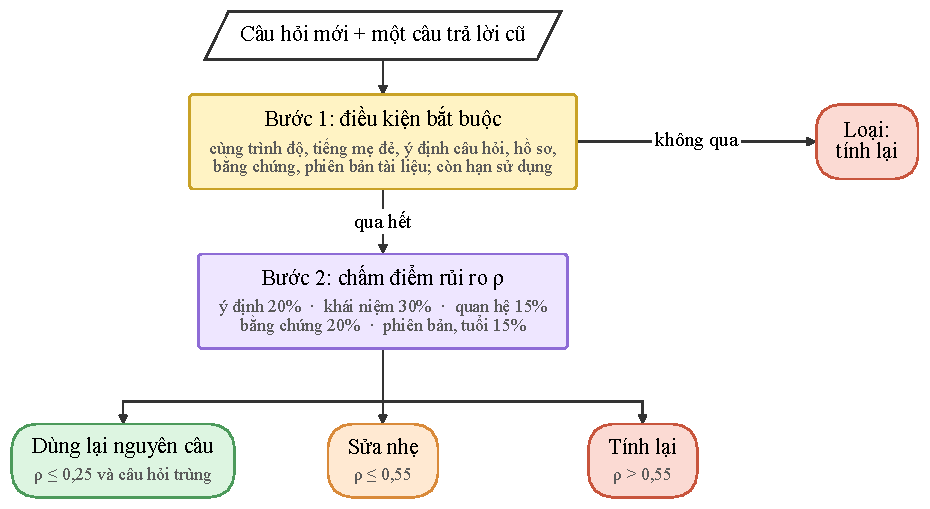
\includegraphics{figures/tracecag/h04_chung_chi.pdf}
  \caption{Kiểm chứng chỉ (\texttt{decide\_l1\_reuse}): điều kiện bắt buộc trước, điểm rủi ro $\rho$ sau.}
  \label{fig:tc-chungchi}
\end{figure}

\begin{figure}[htbp]
  \centering
  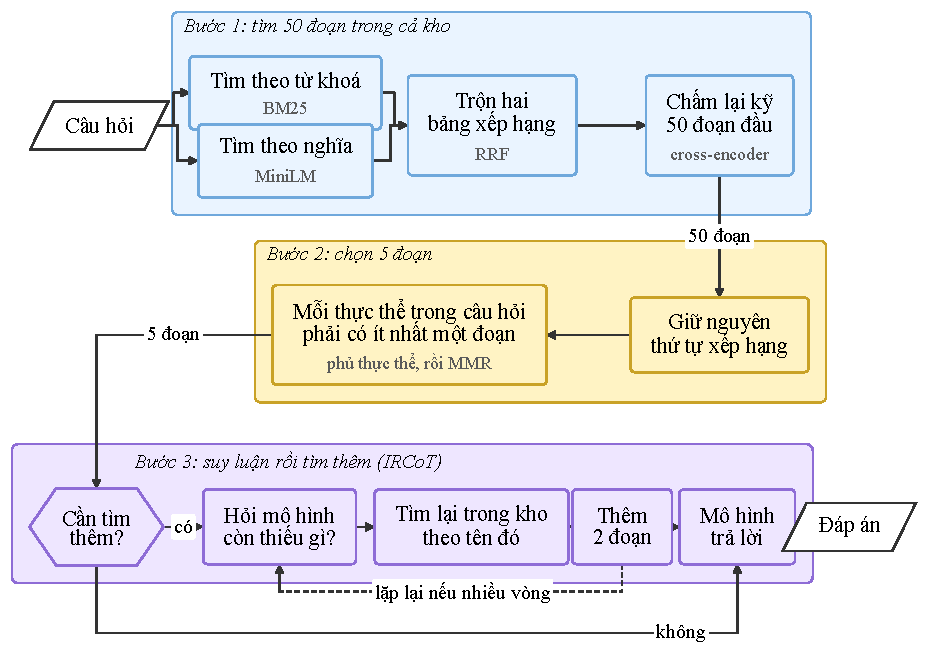
\includegraphics{figures/tracecag/h05_truy_hoi_benchmark.pdf}
  \caption{Tìm bằng chứng cho câu hỏi nhiều bước trong cấu hình chính khi đo trên MuSiQue: tìm 50 đoạn, chọn 5, rồi IRCoT tìm thêm một lần.}
  \label{fig:tc-truyhoibench}
\end{figure}

\begin{figure}[htbp]
  \centering
  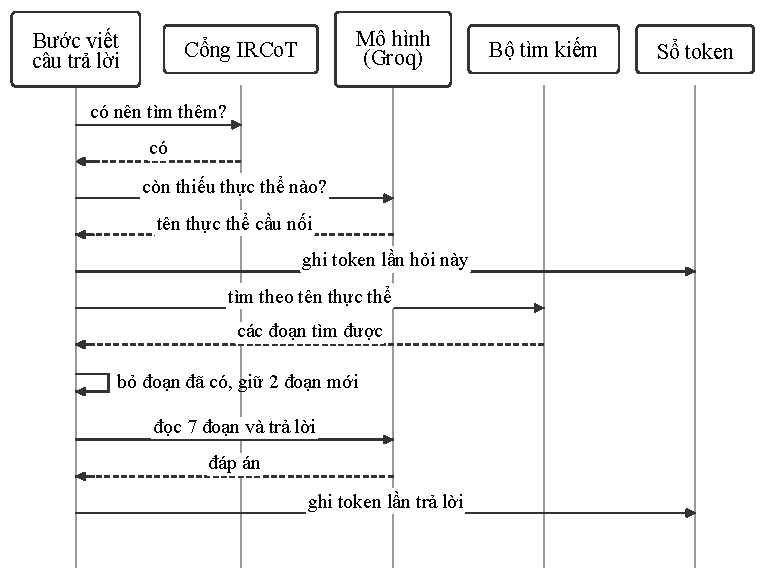
\includegraphics{figures/tracecag/h06_ircot.pdf}
  \caption{Một vòng IRCoT: mô hình được hỏi hai lần, cả hai lần đều ghi vào sổ token.}
  \label{fig:tc-ircot}
\end{figure}

\begin{figure}[htbp]
  \centering
  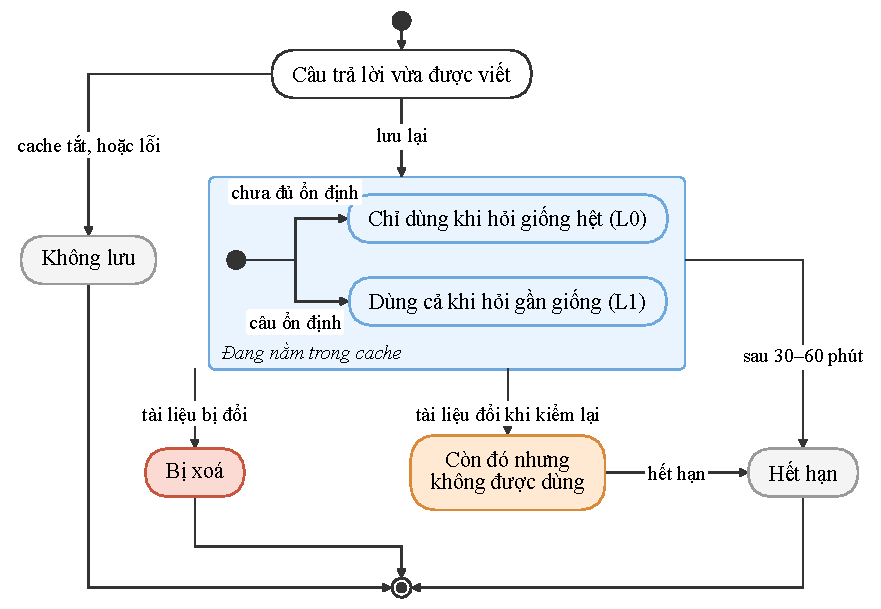
\includegraphics{figures/tracecag/h07_vong_doi.pdf}
  \caption{Vòng đời một câu trả lời trong cache.}
  \label{fig:tc-vongdoi}
\end{figure}

\begin{figure}[htbp]
  \centering
  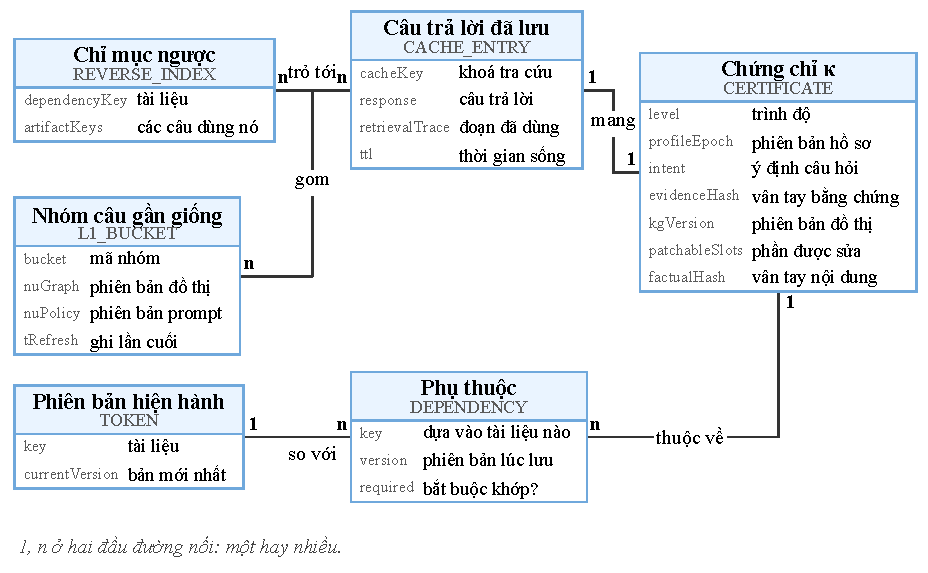
\includegraphics{figures/tracecag/h08_du_lieu.pdf}
  \caption{Dữ liệu của cache: câu trả lời, chứng chỉ $\kappa$ và các phụ thuộc; chỉ mục ngược cho biết câu nào phải xoá khi một tài liệu đổi.}
  \label{fig:tc-dulieu}
\end{figure}

\begin{figure}[htbp]
  \centering
  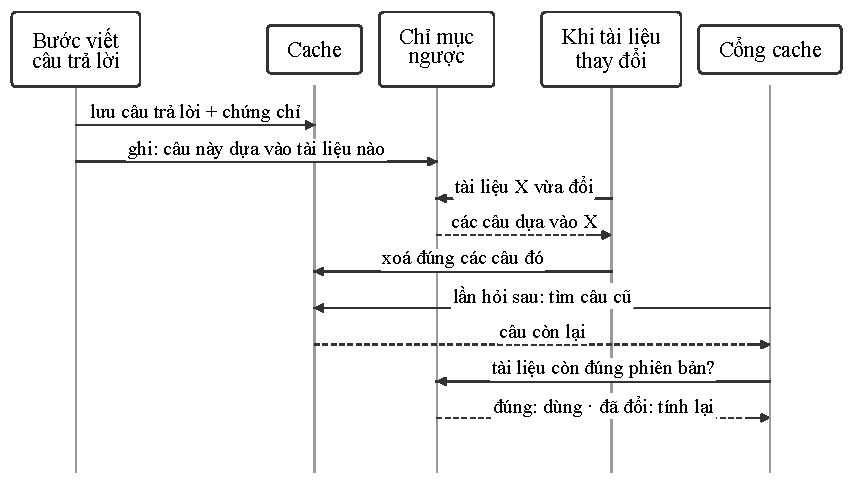
\includegraphics{figures/tracecag/h09_vo_hieu_hoa.pdf}
  \caption{Khi tài liệu đổi, chỉ những câu trả lời dựa vào nó bị xoá; trước khi dùng lại, phiên bản được kiểm thêm một lần.}
  \label{fig:tc-vohieuhoa}
\end{figure}

\begin{figure}[htbp]
  \centering
  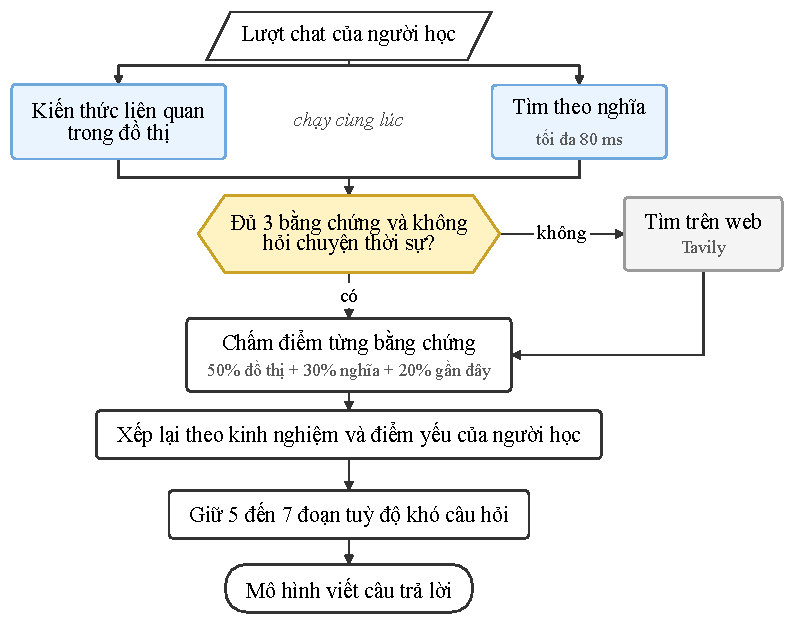
\includegraphics{figures/tracecag/h10_truy_hoi_production.pdf}
  \caption{Tìm bằng chứng trong ứng dụng chat: đồ thị kiến thức và tìm theo nghĩa chạy cùng lúc; web chỉ khi cần.}
  \label{fig:tc-truyhoiprod}
\end{figure}

\begin{figure}[htbp]
  \centering
  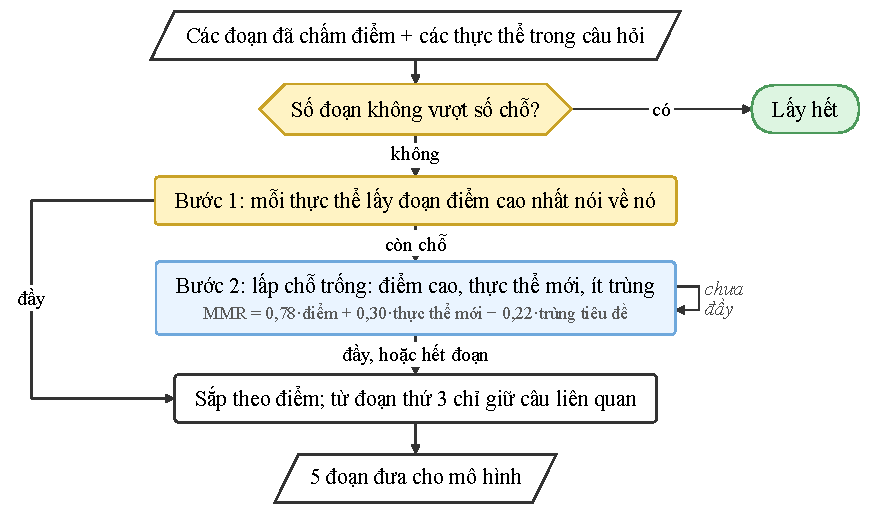
\includegraphics{figures/tracecag/h11_chon_cua_so.pdf}
  \caption{Chọn 5 đoạn: mỗi thực thể trong câu hỏi giữ một chỗ trước, chỗ còn lại theo MMR.}
  \label{fig:tc-cuaso}
\end{figure}

\begin{figure}[htbp]
  \centering
  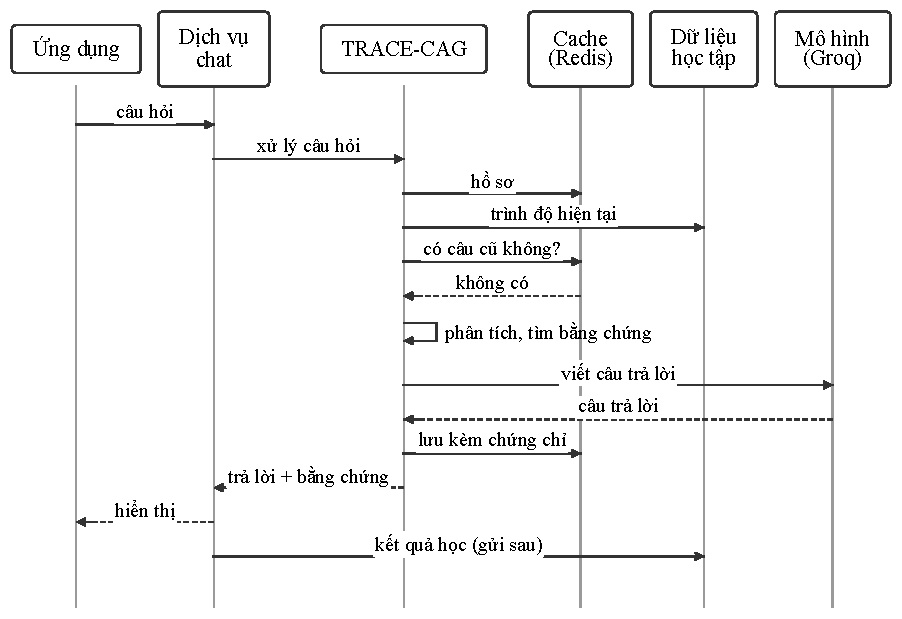
\includegraphics{figures/tracecag/h12_luot_chat.pdf}
  \caption{Một lượt chat khi không có câu trả lời cũ dùng lại được.}
  \label{fig:tc-luotchat}
\end{figure}

\begin{figure}[htbp]
  \centering
  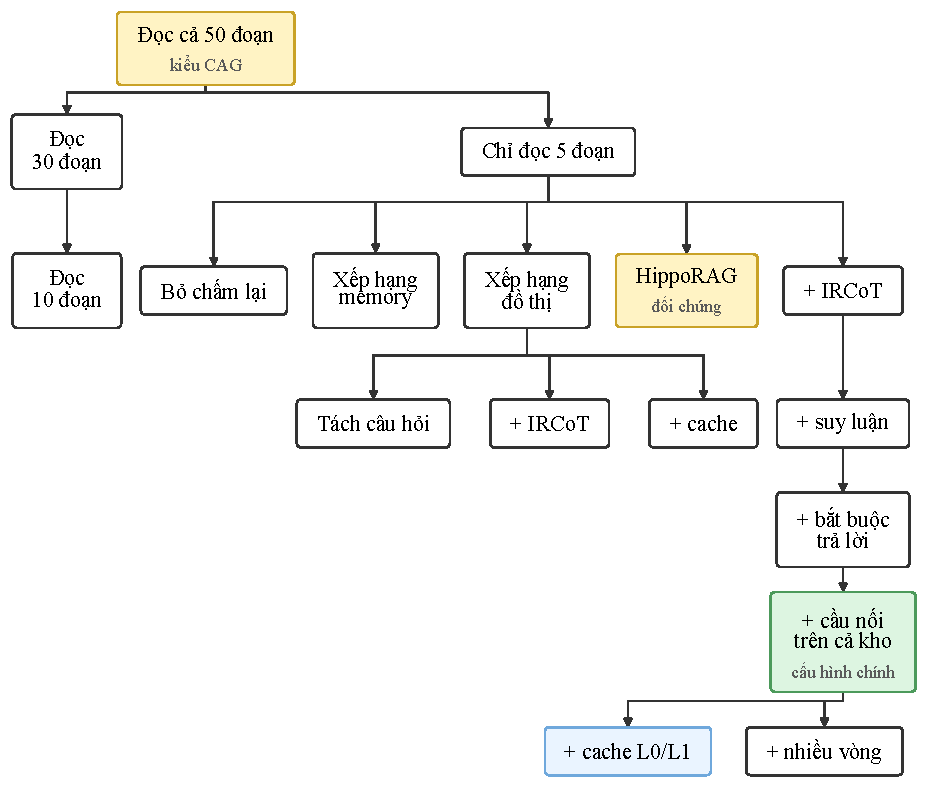
\includegraphics{figures/tracecag/h13_cay_nhanh.pdf}
  \caption{Các cấu hình được so sánh khi đo; mỗi mũi tên đổi đúng một thiết lập so với ô trước.}
  \label{fig:tc-caynhanh}
\end{figure}
